
%(BEGIN_QUESTION)
% Copyright 2007, Tony R. Kuphaldt, released under the Creative Commons Attribution License (v 1.0)
% This means you may do almost anything with this work of mine, so long as you give me proper credit

Inspecting the trends of PV and SP on a process chart recorder, you notice the poor quality of control:

$$\includegraphics[width=15.5cm]{i01646x01.eps}$$

The ``wandering'' of the process variable (PV) around setpoint may be due to excessive action on the part of the controller, or it may be due to load fluctuations in the process itself.  In other words, the instability may be the fault of the controller reacting too aggressively, or it may be that the controller is not working aggressively enough to counter changes in process load.  

Identify a simple method to determine which scenario is true.  Hint: the way to check is as simple as pushing a single button, in most cases.

\underbar{file i01646}
%(END_QUESTION)





%(BEGIN_ANSWER)

Place the controller in manual mode and observe the PV trend!

%(END_ANSWER)





%(BEGIN_NOTES)

If the PV wanders even more with the controller in manual mode, then you know the controller was doing it's job, though perhaps not aggressively enough.  If the PV stops wanders less or stops wandering completely after the controller has been placed in manual mode, then you know the controller's action is actually making matters {\it worse}.

Not all cases of controller over-tuning result in a nice sine-wave oscillation as some textbooks show!  It is possible for an over-tuned controller to exhibit odd trend patterns, especially if the process has asymmetrical time constants (for example, a furnace that heats up faster than it cools down).

Also, it {\it is} possible for the PV to oscillate in a nice sine-wave pattern and not have it be the controller's fault.  If another control loop in a system is over-tuned and oscillating, for example, it may load the process you're observing with a sine-wave disturbance, causing many process variables throughout the system to ``ripple'' correspondingly.  
 
%INDEX% Control, PID tuning: manual mode as a diagnostic tool

%(END_NOTES)


